\begin{figure}[t]
  \centering
\begin{tikzpicture}

\node[inner sep=0pt] (img) at (0 - 3.0cm, 0.0 + 0.3cm)
    {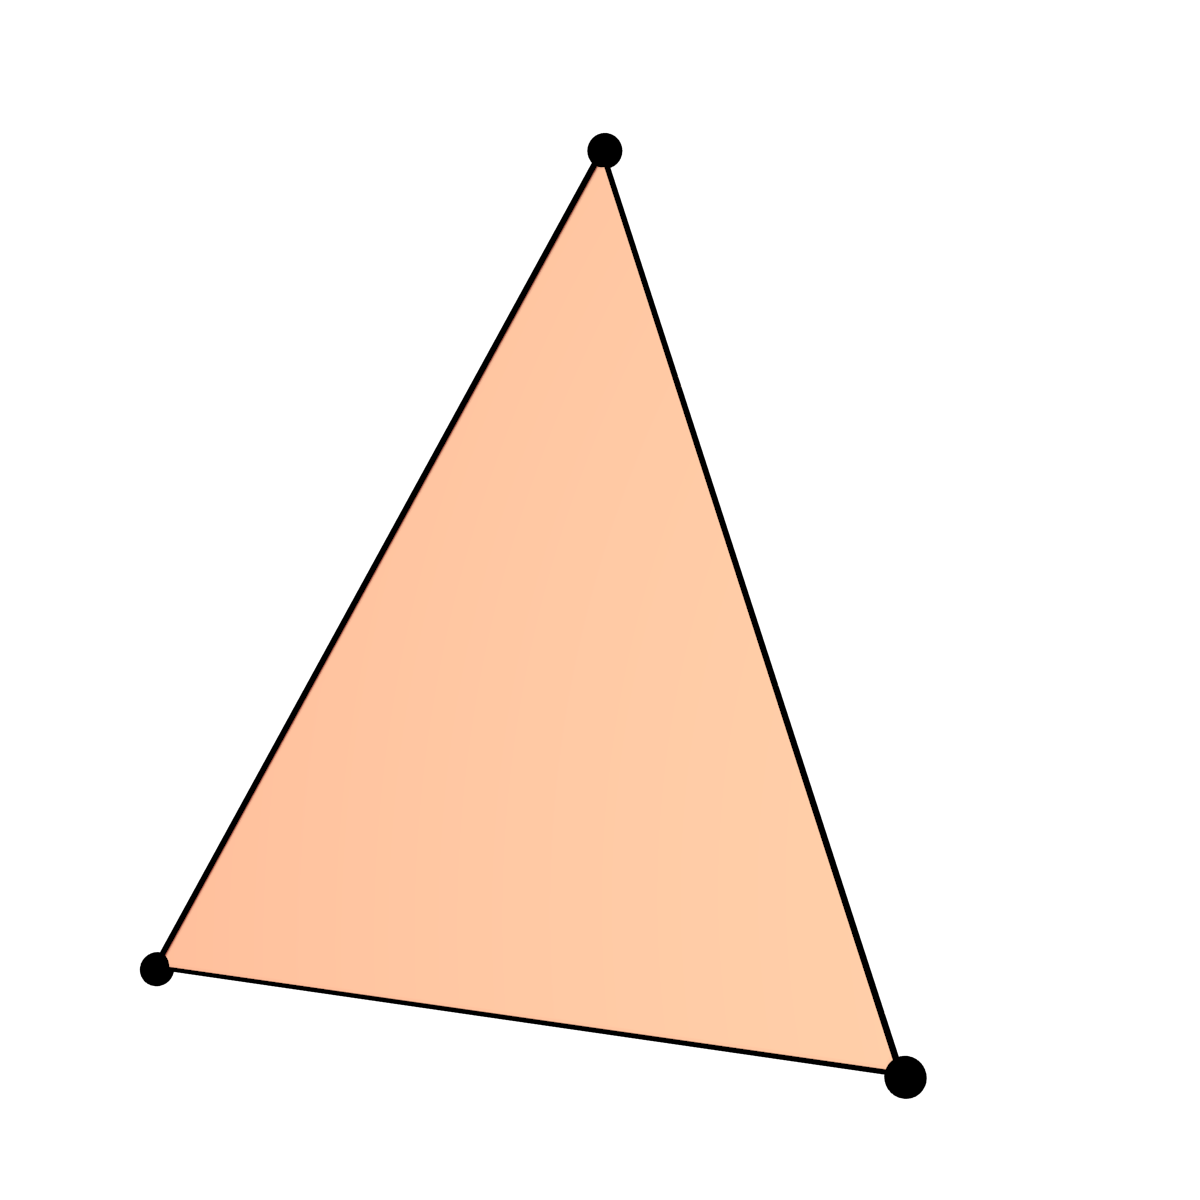
\includegraphics[width=2.5cm]{./img/raw/gd-object-triangle.png}};

\node (l1) at ( 0.8cm - 3.0cm, -1.3cm + 0.3cm) {$\mathbf{v_1}$};
\node (l2) at ( -1.1cm - 3.0cm, -1.05cm + 0.3cm) {$\mathbf{v_2}$};
\node (l3) at ( 0.0cm - 3.0cm,  1.2cm + 0.3cm) {$\mathbf{v_3}$};

\node[inner sep=0pt] (img) at (-0.5cm - 3cm, -4.0cm)
    {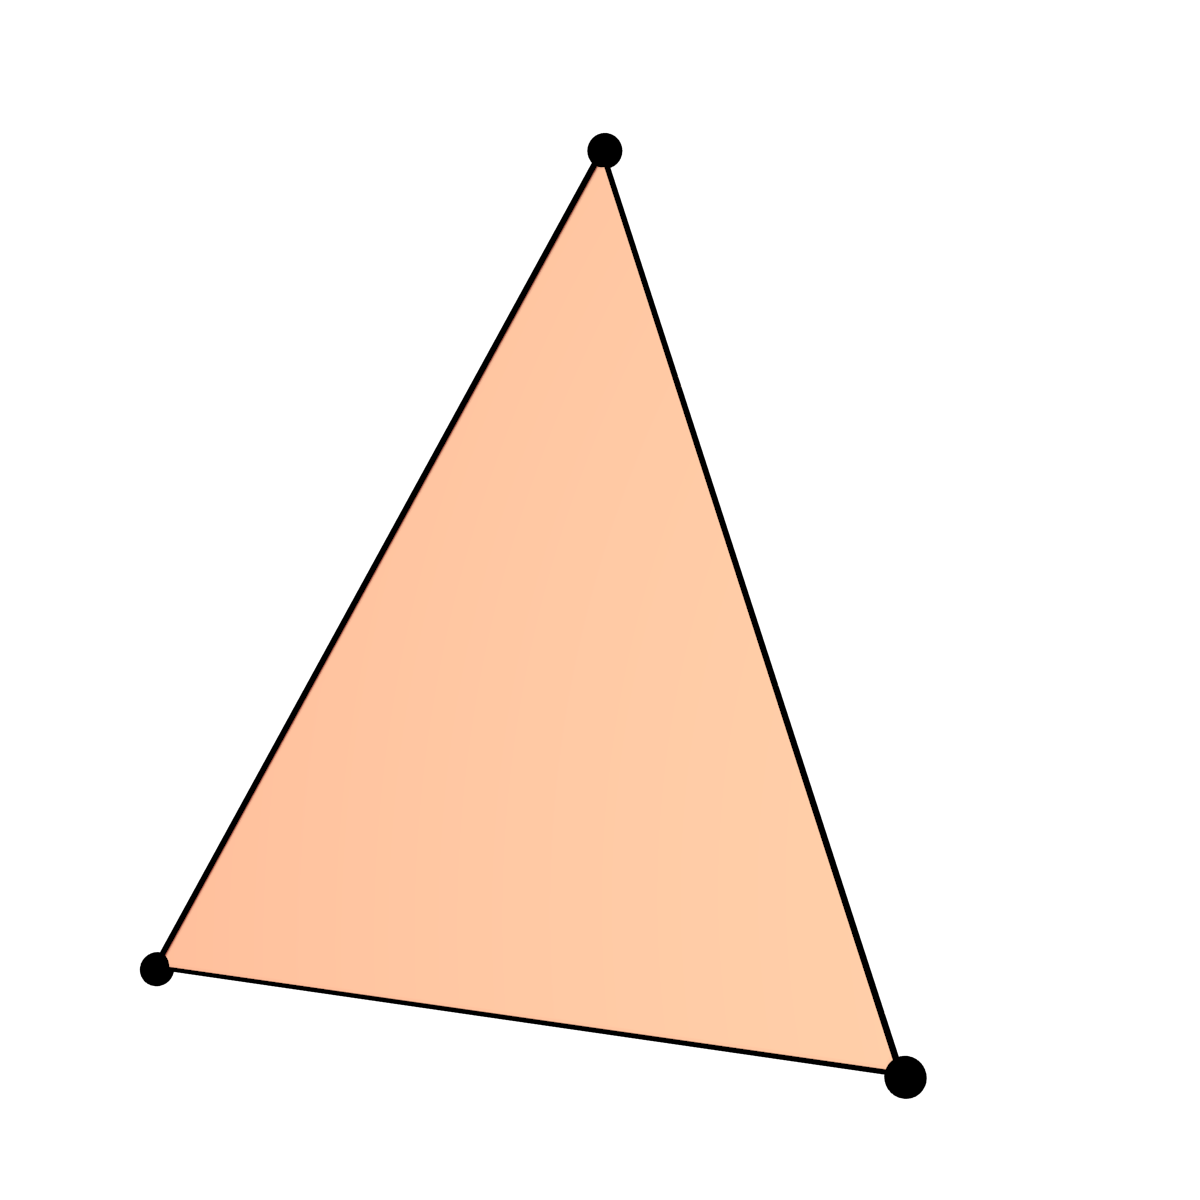
\includegraphics[width=2.5cm]{./img/raw/gd-object-triangle.png}};
\node[inner sep=0pt] (img) at (-0.25cm - 3cm, -4.25cm)
    {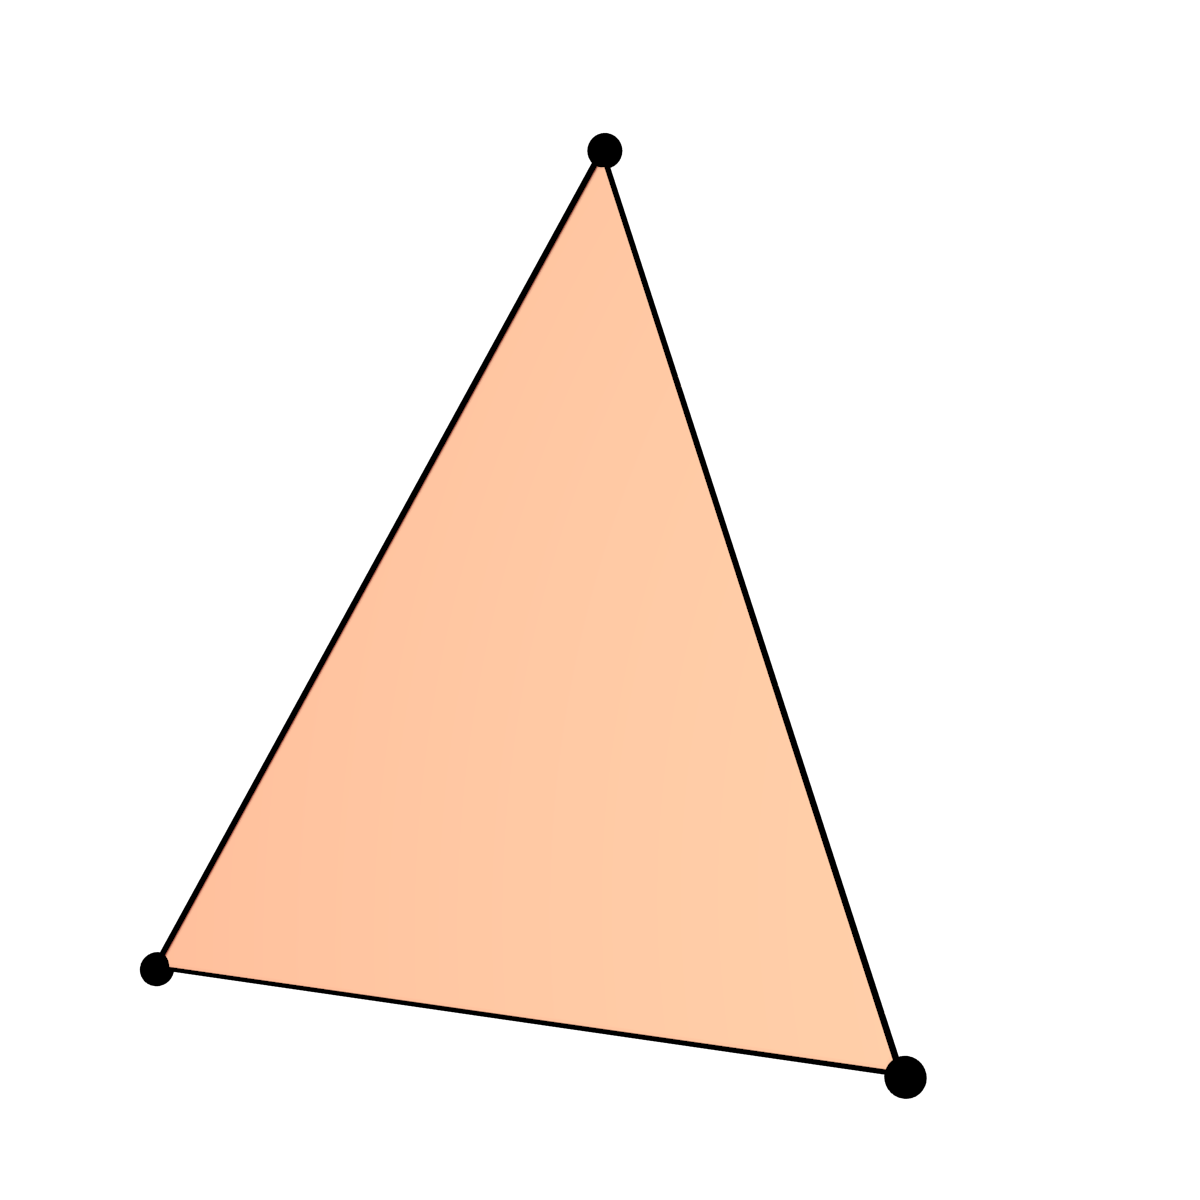
\includegraphics[width=2.5cm]{./img/raw/gd-object-triangle.png}};
\node[inner sep=0pt] (img) at (0  - 3cm, -4.5cm)
    {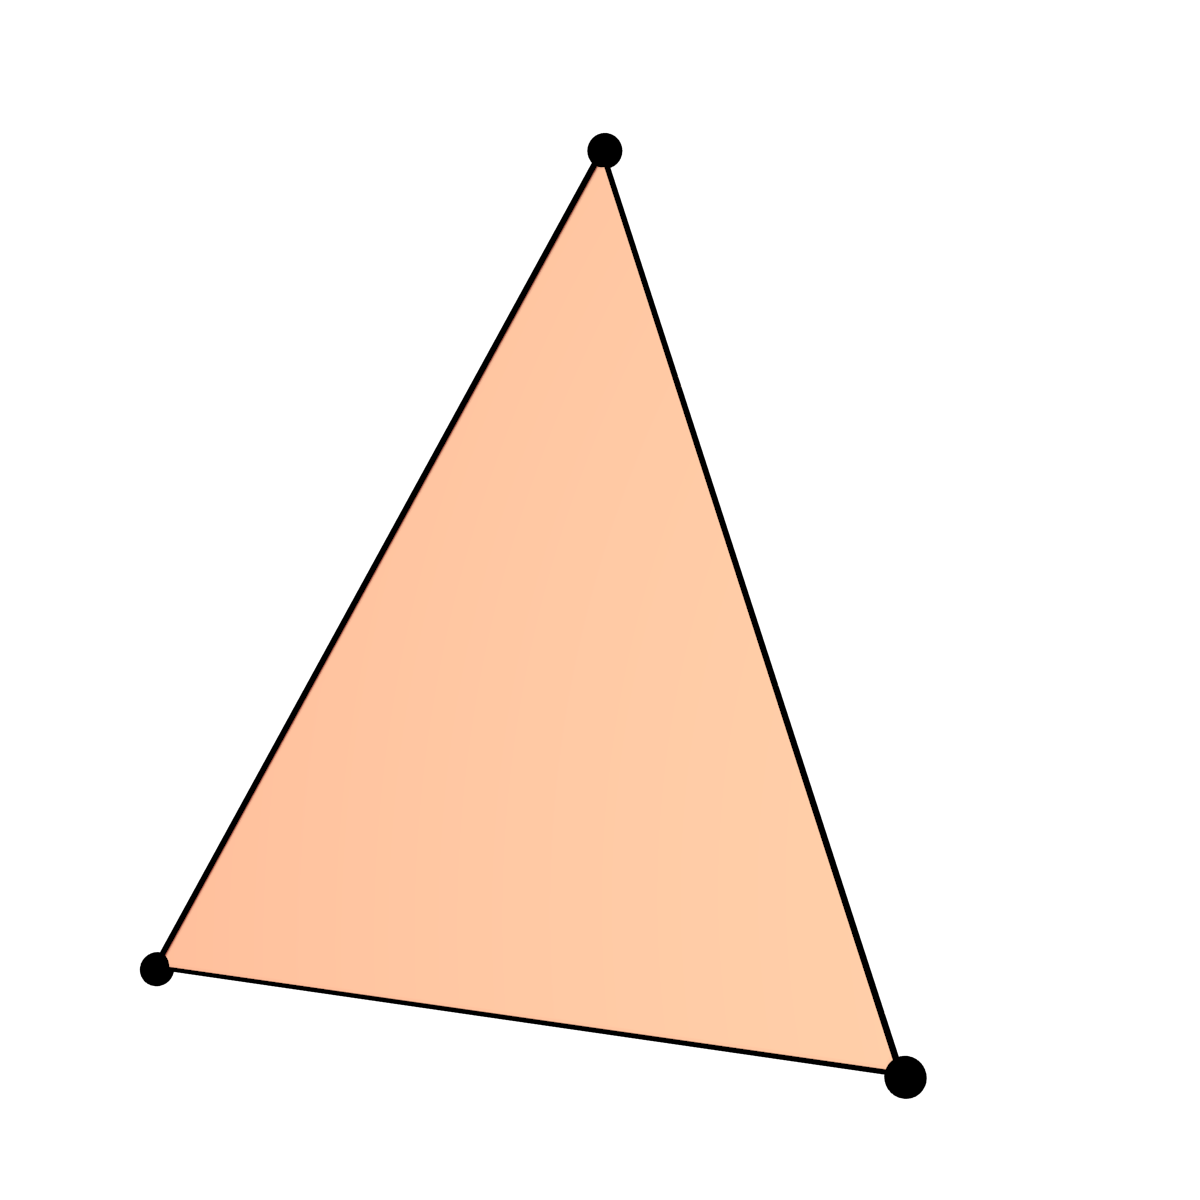
\includegraphics[width=2.5cm]{./img/raw/gd-object-triangle.png}};
\node (l3) at (-3.2cm, -4.25cm) [rectangle, minimum height=4.0cm, minimum width=4.0cm, draw=black, rounded corners=2.5, ] {};

\node[inner sep=0pt] (img) at (0  + 2cm, -4.3cm)
    {\includegraphics[width=4.0cm]{./img/raw/gd-object-mesh.png}};
\node at (-1cm,-4.3cm) [] () {:};

\node[inner sep=0pt] (img) at (0  - 3cm, -9.25cm)
    {\includegraphics[width=3.0cm]{./img/raw/gd-object-mesh.png}};
\node at (-1cm,-10cm) [] () {:};
\node[inner sep=0pt] (img) at (0  + 2.5cm, -10cm)
    {\includegraphics[width=6.0cm]{./img/raw/gd-object-obj.png}};
\node (l3) at (-3.2cm, -11.75cm) {$\lbrace A_1, A_2, A_3, A_4 \rbrace$};

\node (l3) at (-3.2cm, -10cm - 0.125cm) [rectangle, minimum height=5.25cm, minimum width=4.0cm, draw=black, rounded corners=2.5, ] {};
\node (l3) at (-3.2cm, 0.275cm) [rectangle, minimum height=3.5cm, minimum width=4.0cm, draw=black, rounded corners=2.5, ] {};

\node (a1) at (0.0cm  - 3.0cm, -1.4cm) [] {};
\node (a2) at (0.0cm  - 3.0cm, -2.4cm) [] {};
\draw[-latex] (a1) -- (a2);

\node (a1) at (-3.0cm, -1.2cm - 4.95cm) [] {};
\node (a2) at (-3.0cm, -2.0cm - 5.65cm) [] {};
\draw[-latex] (a1) -- (a2);

\node at (-5.75cm, 0.15cm) [rotate=90] {Primitief};
\node at (-5.75cm, 0.15cm - 4.3cm) [rotate=90] {Mesh};
\node at (-5.75cm, 0.15cm - 9.75cm) [rotate=90] {Object};

%\node[inner sep=0pt] (img1) at (0.0, 0.0)
%    {\includegraphics[width=0.25\textwidth]{gd-object-mesh.png}};
%\node (l2) at (0.0, -3) {Mesh};
    
%\node (l3) at (0.0, -5) {$\lbrace A_1, A_2, A_3, A_4 \rbrace \text{ where } A_i =  
%\begin{bmatrix}
  %a_{1,1} & a_{2,1} & a_{3,1} & a_{4, 1} \\
  %a_{1,2} & a_{2,2} & a_{3,2} & a_{4, 2} \\
  %a_{1,3} & a_{2,3} & a_{3,3} & a_{4, 3} \\
  %a_{1,4} & a_{2,4} & a_{3,4} & a_{4, 4} \\
 %\end{bmatrix} $};
%\node (l3) at (0.0, -6.5) {Transformation matrices per object};

%\draw[-stealth, thick] (5,-3.5) -- (7,-3.5);

%\node[inner sep=0pt] (img1) at (14.0, -1.0)
    %{\includegraphics[width=0.6\textwidth]{gd-object-obj.png}};
%\node (l4) at (14.0, -6.5) {Collection of objects};

\end{tikzpicture}

  
  \caption{Voorstelling van objecten door middel van driehoeken.}
  \label{fig:gd-object}
\end{figure}

